% ============================================================================
% AOGS MASTER OVERVIEW — one document to explain the whole poster, organized
% BY FIGURE. Consolidates the plain-language explainer + the expert briefing
% into a single figure-walk: for each poster figure — what it shows, the
% physics behind it, what to say, and the question it draws.
% Numbers via poster_numbers.tex (generated, never hand-typed).
% Build:  /Library/TeX/texbin/pdflatex aogs_master_overview.tex   (x2)
% ============================================================================
\documentclass[11pt]{article}
\usepackage[a4paper, margin=18mm]{geometry}
\usepackage[T1]{fontenc}
\usepackage{newtxtext,newtxmath}
\usepackage{graphicx}
\usepackage{booktabs}
\usepackage{xcolor}
\usepackage[font=small,labelfont=bf]{caption}
\usepackage{enumitem}
\usepackage{amsmath}
\usepackage{mdframed}
\usepackage{float}
\newcommand{\horAfif}{14.0}
\newcommand{\lossAfif}{1.16}
\newcommand{\svfAfif}{0.985}
\newcommand{\kdstarAfif}{4.60}
\newcommand{\horAsev}{10.1}
\newcommand{\lossAsev}{0.18}
\newcommand{\svfAsev}{0.991}
\newcommand{\kdstarAsev}{7.08}
\newcommand{\rmsehayAfif}{2.03}
\newcommand{\rmsecpAfif}{1.74}
\newcommand{\bestzcpAfif}{5/30}
\newcommand{\bestrhocpAfif}{1500/1700/1700}
\newcommand{\rmsecKAfif}{0.90}
\newcommand{\bestzcKAfif}{10/30}
\newcommand{\bestrhocKAfif}{1500/1700/1800}
\newcommand{\rmsehayAsev}{0.54}
\newcommand{\rmsecpAsev}{0.39}
\newcommand{\bestzcpAsev}{5/30}
\newcommand{\bestrhocpAsev}{1500/1700/1700}
\newcommand{\rmsecKAsev}{0.36}
\newcommand{\bestzcKAsev}{5/30}
\newcommand{\bestrhocKAsev}{1300/1500/1900}
\newcommand{\rmsehomAfif}{2.31}
\newcommand{\rmsehomAsev}{3.76}
\newcommand{\xferatAsev}{1.64}
\newcommand{\xferatAfif}{1.73}
\newcommand{\svfdtirAfif}{1.15}
\newcommand{\svfdtallAfif}{1.30}
\newcommand{\svfdtirAsev}{0.65}
\newcommand{\svfdtallAsev}{0.74}
\newcommand{\shadowcoolAfif}{2.22}
\newcommand{\shadowcoolAsev}{0.48}
\newcommand{\stabcKAfif}{13}
\newcommand{\bootcicKAfif}{0.26--1.08}
\newcommand{\stabcKAsev}{36}
\newcommand{\bootcicKAsev}{0.25--0.43}
\newcommand{\driftmax}{35}
\newcommand{\closurewin}{0.70}


\definecolor{teal}{HTML}{2A6478}
\definecolor{coral}{HTML}{B85B3A}
\definecolor{forest}{HTML}{3D6E4A}
\definecolor{char}{HTML}{2A2520}
\definecolor{gridc}{HTML}{E8E5E0}
\definecolor{dim}{HTML}{8A857E}
\color{char}

\graphicspath{{../figures/poster/}{../figures/diagrams/}{../figures/explainers/}}
\setlist[itemize]{leftmargin=1.3em, itemsep=1pt, topsep=2pt}
\setlist[enumerate]{leftmargin=1.5em, itemsep=1pt, topsep=2pt}

\newcommand{\shead}[1]{\medskip\noindent{\color{teal}\large\bfseries #1}\par
  \nobreak\vspace{-2pt}{\color{teal}\rule{\linewidth}{0.6pt}}\par\smallskip}

% the four-line "explain this figure" card
\newmdenv[linecolor=gridc, linewidth=1pt, backgroundcolor=gridc!35,
          roundcorner=3pt, innertopmargin=5pt, innerbottommargin=6pt,
          innerleftmargin=7pt, innerrightmargin=7pt, skipabove=4pt]{card}
\newcommand{\shows}{\textbf{\color{teal}Shows.}\ }
\newcommand{\phys}{\textbf{\color{forest}Physics.}\ }
\newcommand{\say}{\textbf{\color{char}Say / point at.}\ }
\newcommand{\expect}{\textbf{\color{coral}Expect the question.}\ }

\begin{document}
\thispagestyle{empty}

\begin{center}
{\LARGE\bfseries The AOGS Poster --- Master Overview}\\[2pt]
{\large\color{teal}\bfseries Everything happening in every figure, in one place}\\[4pt]
{\small Ram\'on III P.\ Gregorio \quad$\bullet$\quad Institute of Science Tokyo}\\[-1pt]
{\footnotesize\color{dim} \emph{Discrete Layer Thermal Modeling of Lunar Landing
 Sites with Topographic Shadowing} \quad$\bullet$\quad every number from the results archives}
\end{center}
\vspace{1pt}{\color{teal}\rule{\linewidth}{0.9pt}}

% ── STORY ────────────────────────────────────────────────────────────────────
\shead{The study in five sentences}
The only in-situ measurements of the lunar subsurface thermal state are the
Apollo 15 and 17 Heat Flow Experiment (HFE) records. We take a certified 1-D
thermal-diffusion model of those sites and add two pieces of physics the
standard description lacks: \textbf{discrete density layers} (instead of the
smooth exponential of Hayne et al.\ 2017) and \textbf{topographic shadowing}
ray-traced from the LOLA elevation model. Sweeping 650 layer configurations
against the deep sensors shows the record prefers a surface denser than
Hayne's surface value and a shallow transition to consolidated regolith --- and
the fit improves not because density stores heat differently, but because
density \emph{implies conductivity} through the model's own $K_c(\rho)$
relation. The retrieved deep densities (1800/1900 kg\,m$^{-3}$) match the
Apollo drive cores (${\sim}$1825/1960; Grott et al.) in magnitude and site
ordering. Topography enters twice through opposing channels of comparable
size --- horizon blocking cools the deep sensors
(\shadowcoolAfif/\shadowcoolAsev\ K), terrain re-radiation warms them
($+\svfdtallAfif$/$+\svfdtallAsev$ K upper bound) --- so neither can be
dismissed on the assumption the other cancels it.

% ── CLAIM LADDER ─────────────────────────────────────────────────────────────
\shead{The claim ladder --- never defend a rung above the evidence}
\begin{enumerate}
  \item \textbf{Strong:} the deep-sensor record is reproduced to
    \rmsecKAfif/\rmsecKAsev\ K by a 3-layer column; the conductivity channel
    dominates the heat-capacity channel (${\sim}4$ K vs $<0.8$ K of leverage);
    the two topographic channels are each ${\gtrsim}1$ K-scale and oppose.
  \item \textbf{Solid:} the improvement is bootstrap-robust (coupled 95\% CIs
    \bootcicKAfif/\bootcicKAsev\ K, below homogeneous \rmsehomAfif/\rmsehomAsev\
    K); retrieved deep densities match the drive cores.
  \item \textbf{Scoped (say the qualifier first):} vs.\ the \emph{field-standard}
    Hayne continuous model the gains are ${\sim}2.3\times$ (A15) /
    ${\sim}1.5\times$ (A17) --- the ${\sim}2.6\times/10\times$ figures are vs.\
    homogeneous. At A17 cp (\rmsecpAsev\ K) nearly ties coupled (\rmsecKAsev\ K).
  \item \textbf{Class-level only:} the A15 \emph{exact} triple survives only
    \stabcKAfif\% of bootstrap draws --- claim the class (denser surface,
    shallow transition), never the individual triple.
  \item \textbf{Concede freely:} terrain-radiation numbers are an upper bound
    not yet in the sweep; the 16 ppd DEM under-resolves near-field terrain;
    $K_d$--density degeneracy needs a joint retrieval.
\end{enumerate}

% ── PHYSICS PRIMER ───────────────────────────────────────────────────────────
\shead{The physics in one box (everything the figures rest on)}
\textbf{Heat equation:}
$\rho(z)\,c_p(T)\,\partial_t T=\partial_z[K(T,z)\,\partial_z T]$ --- 1-D vertical
conduction. \textbf{Conductivity (Hayne 2017):}
$K(T,z)=K_c(z)[1+\chi(T/350\,\mathrm{K})^3]$, contact + radiative ($T^3$) parts,
with $K_c(z)=K_d-(K_d-K_s)e^{-z/H}$; $\chi{=}2.7$, $K_s{=}0.74$, $H{=}6$ cm.
\textbf{Boundaries:} surface
$(1{-}A)S_{\rm sh}=\varepsilon\sigma T_s^4+K\partial_z T|_0$; base
$K\partial_z T|_{\rm deep}=Q_b=21/16$ mW\,m$^{-2}$ (A15/A17). \textbf{Shadowing:}
$S_{\rm sh}=(1{-}A)S_0\cos\theta_s$ if the Sun is above the DEM skyline
$\theta_h(\varphi)$, else $0$. \textbf{The two branches:} \textbf{cp} holds
$K_d=K_d^{\star}$ (\kdstarAfif/\kdstarAsev\ mW\,m$^{-1}$K$^{-1}$) and lets
density move only $c_p$; \textbf{coupled} sets $K_d=K_c(\rho_3)$ from the line
through $(\rho_s{=}1100,K_s)$ and $(\rho_d{=}1800,K_d^{\star})$ --- no new
constants. \textbf{Score:} RMSE of the equilibrium mean profile
$\overline{T}(z_i)$ against the deep sensors (0.8--2.4 m).

\medskip
\noindent\textbf{The one subtlety that runs through the whole poster --- the
degeneracy.} The deep gradient is essentially $Q_b/K_{\rm deep}$, and
\emph{both} a higher $K_d$ and a denser deep layer raise $K_{\rm deep}$. So the
sensors cannot separate them: the letter pinned density (Hayne) and retrieved
$K_d^{\star}$; this study pins $K_d^{\star}$ and retrieves density --- two
conditional slices of one coupled space. In the coupled branch the winner's
\emph{effective} deep conductivity is $K_c(\rho_3)$: A15's $\rho_3{=}1800$ gives
4.60 (unchanged), A17's $\rho_3{=}1900$ gives 7.99 ($+0.91$ above the anchor).
That is not a contradiction --- it is the degeneracy, and the honest framing.

\clearpage
% ══════════════════ FIGURE WALK ═════════════════════════════════════════════
\shead{Figure walk --- explain each panel}
The rest of this document is one block per poster figure. Read the card, then
the figure; at the board, point at the thing named in \emph{Say}.

% ---- FIG 1 : schematic -------------------------------------------------------
\noindent\textbf{\large Figure 1 --- the physical model}
\begin{card}
\shows a single regolith column: three density layers (loose skin
$\to$ intermediate $\to$ consolidated), the Sun blocked by a massif on the
left, and the borehole with its deep HFE sensors on the right.\\[3pt]
\phys this is the geometry the heat equation runs in. The layers are the
first advance; the blocked Sun (horizon angle $\theta_h$) is the second.
Fluxes shown: absorbed sunlight in, thermal emission out, geothermal $Q_b$
up from below.\\[3pt]
\say point at the two numbered tags --- ``these two, layers and shadowing,
are the contribution; everything else is the certified baseline.''\\[3pt]
\expect \emph{Why three layers?} The coarsest structure that holds a loose
skin, a transition, and a compact base; boundaries and densities are swept,
not assumed.
\end{card}
\begin{figure}[H]\centering
  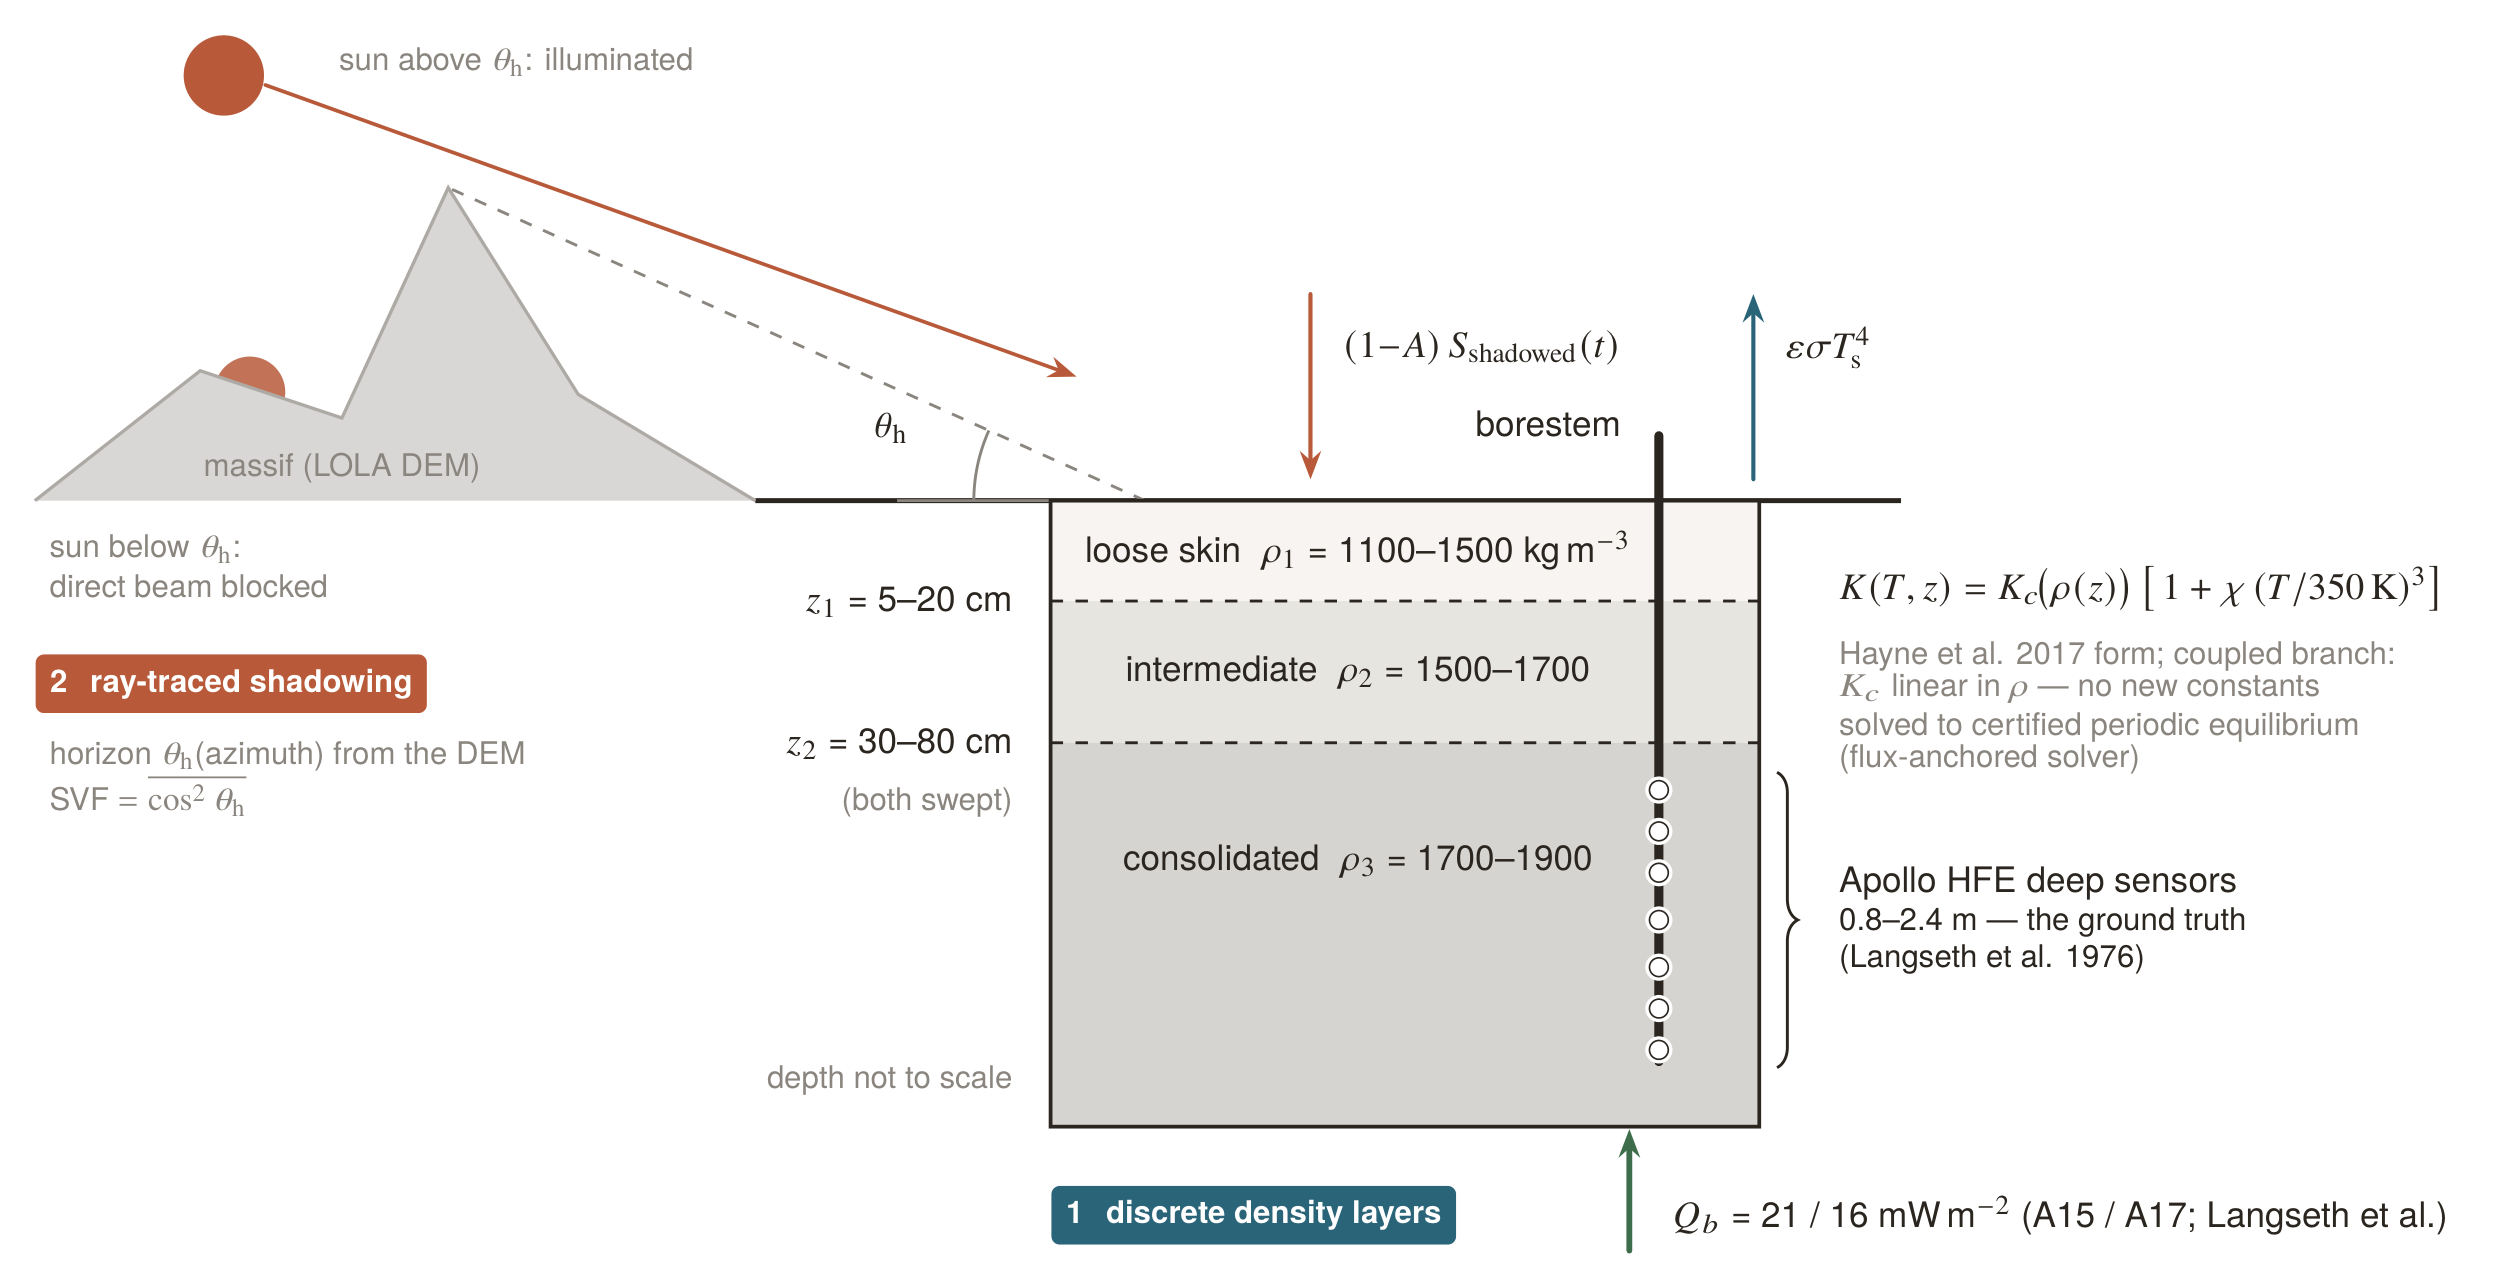
\includegraphics[width=0.70\linewidth]{aogs_model_schematic.pdf}
\end{figure}

% ---- FIG 2 : pipeline --------------------------------------------------------
\noindent\textbf{\large Figure 2 --- how it computes (the pipeline)}
\begin{card}
\shows three inputs (LOLA DEM, Hayne model, Apollo record) feeding a
five-step chain: ray-traced horizons $\to$ 3-layer density $\to$
equilibrium solver $\to$ mean profile $\to$ RMSE, looped over 650
configurations. Teal boxes are new; grey are the certified baseline.\\[3pt]
\phys every box carries its equation. \textbf{Step 2 is the one to know
cold:} it states $K_d^{\star}$ is \emph{site-specific}
(\kdstarAfif/\kdstarAsev), that cp holds it fixed, and that coupled sets
$K_d=K_c(\rho_3)$ anchored at $K_c(1800){=}K_d^{\star}$.\\[3pt]
\say walk the arrows once, top to bottom; rest a finger on the teal/grey
legend --- ``the colour tells you exactly what's new.''\\[3pt]
\expect \emph{Isn't the anchor circular?} See the degeneracy note and the
Q\&A --- the cp branch carries the same anchor and still fails, so the gain is
the profile \emph{shape}, not the anchor.
\end{card}
\begin{figure}[H]\centering
  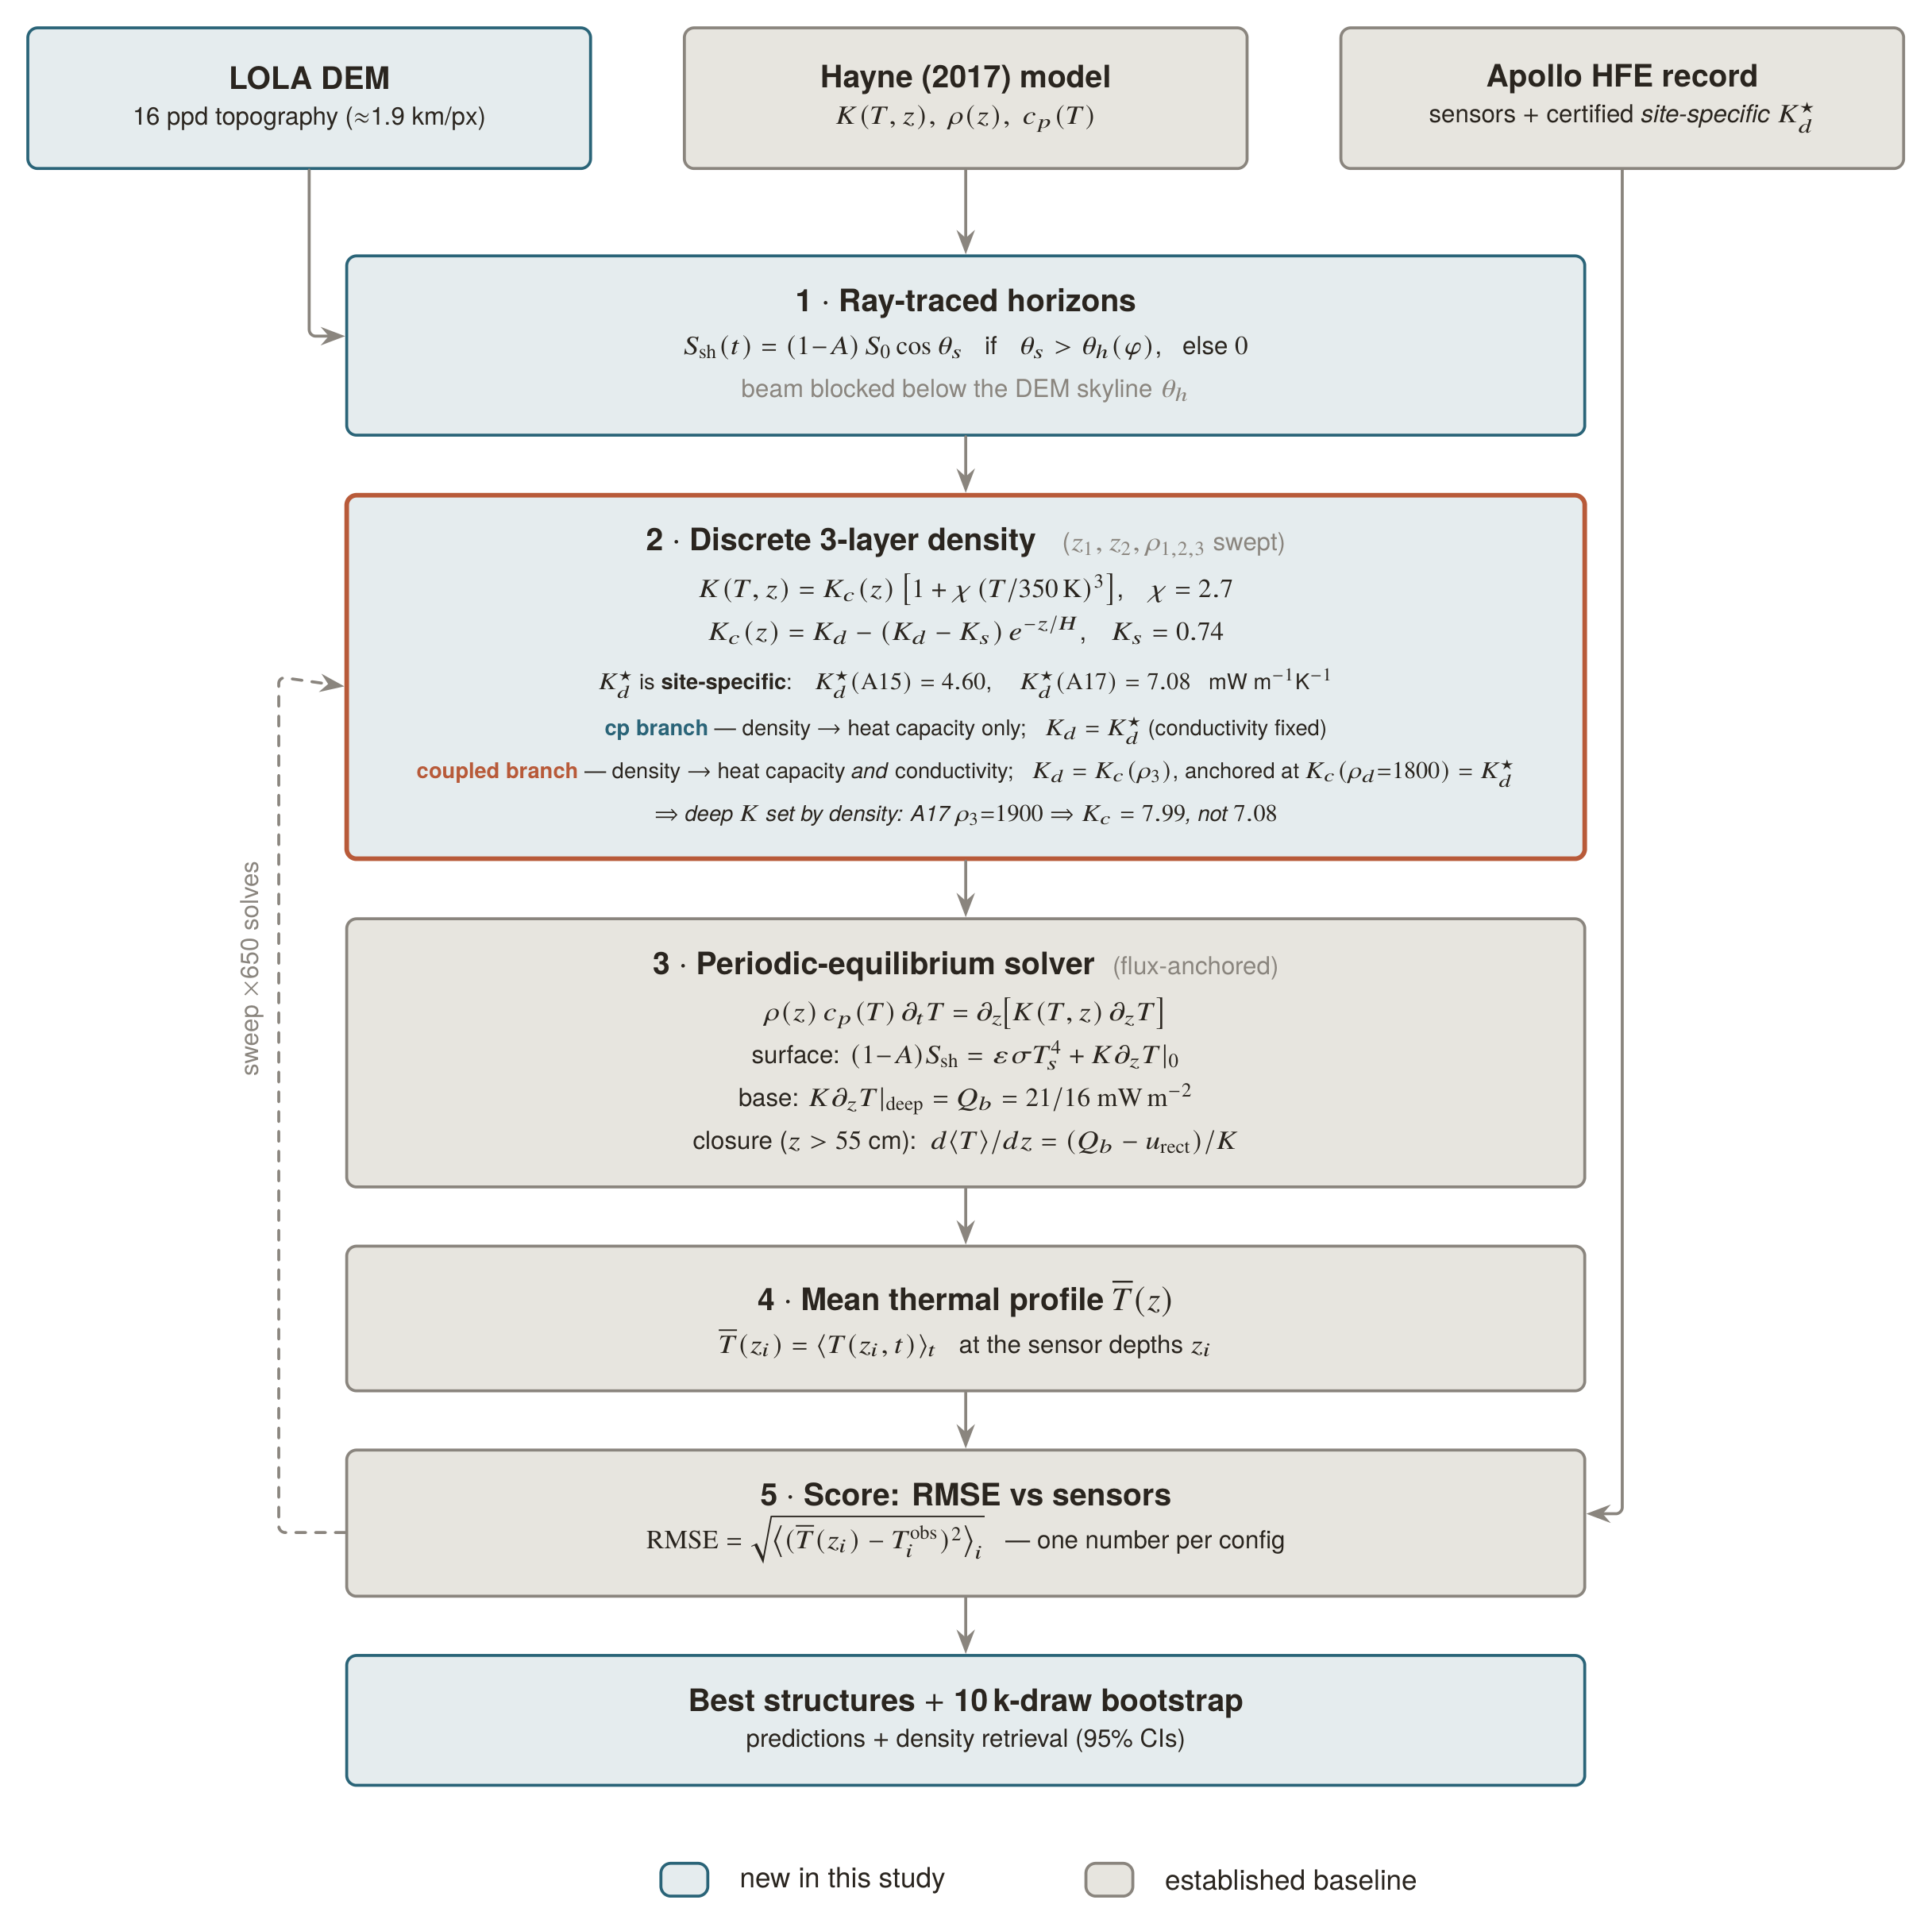
\includegraphics[width=0.58\linewidth]{aogs_pipeline_flowchart.pdf}
\end{figure}

% ---- FIG 3 : densities + transfer --------------------------------------------
\noindent\textbf{\large Figure 3 --- retrieved densities \& the cross-site test}
\begin{card}
\shows \emph{left:} the winning 3-layer density staircases (green A15, coral
A17) against Hayne's smooth dotted curve. \emph{right:} a 2$\times$2 RMSE
matrix --- each site's structure scored at \emph{both} sites.\\[3pt]
\phys the staircases are what the data prefer: denser-than-Hayne surface,
compaction step high in the column. The matrix is a held-out test: the
\emph{diagonal} (\rmsecKAfif/\rmsecKAsev\ K) is each structure at its home
site; the \emph{off-diagonal} (\xferatAfif/\xferatAsev\ K) is transplanted ---
it degrades gracefully and still beats homogeneous.\\[3pt]
\say left staircase vs the dotted line: ``the record wants more density up
here.'' Then the matrix diagonal vs off-diagonal: ``structure travels
between sites --- geology, not curve-fitting.''\\[3pt]
\expect \emph{Concede first:} at A17 the transplanted structure does not beat
Hayne continuous (\rmsehayAsev\ K) --- the transfer argument is strongest at
A15 (\xferatAfif\ K vs Hayne's \rmsehayAfif\ K).
\end{card}
\begin{figure}[H]\centering
  \includegraphics[width=0.80\linewidth]{poster_density.pdf}\hfill
\end{figure}
\vspace{-6pt}
\begin{figure}[H]\centering
  \includegraphics[width=0.44\linewidth]{poster_transfer.pdf}
\end{figure}

% ---- TABLE 1 -----------------------------------------------------------------
\noindent\textbf{\large Table 1 --- the RMSE ladder}
\begin{card}
\shows deep-sensor RMSE for models of increasing physics, both sites.\\[3pt]
\phys read it top-to-bottom as ``more physics, better fit.'' Homogeneous is
the floor; Hayne continuous is the field standard; cp adds layers through
heat capacity; coupled adds layers through conductivity.\\[3pt]
\say have \emph{both} ratios ready --- vs homogeneous ${\sim}2.6\times/10\times$;
vs Hayne ${\sim}2.3\times/1.5\times$. Lead with the honest one if pressed.\\[3pt]
\expect \emph{The $10\times$ is against a straw man.} True --- that is why the
Hayne row is on the poster. The interesting asymmetry: Hayne already fits A17
(\rmsehayAsev\ K) but fails A15 (\rmsehayAfif\ K); layering fixes the site
Hayne cannot.
\end{card}
\begin{table}[H]\centering\small
\begin{tabular}{lcc}
\toprule
model (shadowed forcing) & A15 RMSE (K) & A17 RMSE (K)\\
\midrule
homogeneous (constant $K$, constant $\rho$)     & \rmsehomAfif & \rmsehomAsev\\
Hayne continuous at site $K_d^{\star}$          & \rmsehayAfif & \rmsehayAsev\\
best \textbf{cp} (density $\to$ heat capacity)  & \rmsecpAfif  & \rmsecpAsev\\
best \textbf{coupled} (density $\to$ conductivity) & \textbf{\rmsecKAfif} & \textbf{\rmsecKAsev}\\
\bottomrule
\end{tabular}
\end{table}

% ---- FIG 4 : sensitivity -----------------------------------------------------
\noindent\textbf{\large Figure 4 --- sensitivity: what actually matters}
\begin{card}
\shows \emph{top:} box plots of RMSE across all swept configurations, cp vs
coupled, each site. \emph{bottom:} RMSE over the layer-boundary plane
($z_1$ vs $z_2$), green = good.\\[3pt]
\phys the two boxes are the whole argument in one picture: \emph{same}
density values, two different doors. Through $c_p$ the spread is narrow
($<0.8$ K); through conductivity it is wide (${\sim}4$ K). The maps show
where the boundaries want to sit.\\[3pt]
\say point at the \emph{width} of the two boxes --- ``through heat capacity
nothing happens; through conductivity everything happens.'' Then the green
corner: best fits at $z_2=30$ cm.\\[3pt]
\expect \emph{Say it first:} A17's map has a tied deeper solution, and at A17
cp nearly ties coupled --- the conductivity-lever story is A15-weighted.
\end{card}
\begin{figure}[H]\centering
  \includegraphics[width=0.62\linewidth]{poster_sens.pdf}
\end{figure}

% ---- FIG 5 : profiles --------------------------------------------------------
\noindent\textbf{\large Figure 5 --- validation against the deep sensors}
\begin{card}
\shows modeled mean temperature vs depth for the three model curves, with
the Apollo deep-sensor equilibrium temperatures as open circles, both sites.\\[3pt]
\phys the mechanism is \emph{geometric}: the heat-capacity-only branch can
shift the deep profile up or down but not change its slope; the
density-coupled branch \emph{tilts} the gradient itself onto the sensors ---
which is why it threads points the smooth models miss.\\[3pt]
\say trace the slope of the coupled line through the circles --- ``it
tilts the gradient; the others can only slide a fixed slope.''\\[3pt]
\expect \emph{Why one point per sensor, not the time series?} At 0.8--2.4 m
the diurnal wave is dead; the robust observable is the annual-mean
temperature, taken from quiet late-mission windows.
\end{card}
\begin{figure}[H]\centering
  \includegraphics[width=0.66\linewidth]{poster_profiles.pdf}
\end{figure}

% ---- FIG 6 : bootstrap -------------------------------------------------------
\noindent\textbf{\large Figure 6 --- robustness (bootstrap)}
\begin{card}
\shows best-RMSE 95\% confidence intervals for cp and coupled at each site,
from 10{,}000 draws that resample the sensors and their noise; the
homogeneous baseline is the dashed line (A15) / off-scale arrow (A17).\\[3pt]
\phys the whole interval sitting left of the baseline means the improvement
is not an artefact of any single sensor. The A15 cp interval (upper end
2.17 K) sits close to homogeneous (\rmsehomAfif\ K) --- the robust statement
is about the \emph{coupled} branch.\\[3pt]
\say point at the gap between the coloured intervals and the baseline ---
``resample the data 10\,000 ways, the layered fit still wins.''\\[3pt]
\expect \emph{If the A15 triple survives only \stabcKAfif\% of draws, what
did you retrieve?} A class, with quantified stability: the pattern recurs
across draws even when the exact numbers trade --- point estimates in the
figure, class-level claims in the conclusions.
\end{card}
\begin{figure}[H]\centering
  \includegraphics[width=0.80\linewidth]{poster_bootstrap.pdf}
\end{figure}

\medskip
\noindent\emph{Two supporting figures you may also be asked about:} the
\textbf{sites map} (Fig on the poster's left column) shows the real A15/A17
locations and their ray-traced polar horizons --- Apollo 15 under the
Apennine front (horizon to \horAfif$^\circ$, \lossAfif\% of sunlight lost),
Apollo 17 by the North Massif (\horAsev$^\circ$, \lossAsev\%). The
\textbf{schematic's} SVF fine print ($\mathrm{SVF}=\overline{\cos^2\theta_h}$,
\svfAfif/\svfAsev) is the fraction of open sky; its complement is the terrain
that supplies the warming channel.

\clearpage
% ── DEEP DIVE : DENSITY SWEEP FROM ZERO ──────────────────────────────────────
\shead{Deep dive --- the density sweep, explained from zero}
\emph{If someone asks ``what exactly did you do to find the density?'', this is
the answer, built up from nothing. It underlies Figure 3 and Table 1.}

\medskip
\noindent\textbf{1. Read the axes.} The plot below has \textbf{density} across
the bottom --- how tightly packed the ground is (left = loose/fluffy,
right = compact/heavy, in kg\,m$^{-3}$) --- and \textbf{depth} down the side,
\emph{increasing downward} (0 at the surface, 1 metre at the bottom). So moving
down the plot means digging deeper.

\smallskip
\noindent\textbf{2. A line is a ``density profile.''} It says how packed the
ground is at every depth. Like digging a hole and measuring the dirt at each
level: loose on top, more compact below, because material settles under its own
weight.

\smallskip
\noindent\textbf{3. We describe the ground as three layers.} Instead of a
smooth curve, we use a \textbf{staircase}: a loose \emph{surface skin}
(density $\rho_1$), a \emph{middle} layer ($\rho_2$), and a compact \emph{deep}
layer ($\rho_3$). Two depths mark where the layers change: $z_1$ (skin$\to$mid)
and $z_2$ (mid$\to$deep). On the plot each profile is a staircase stepping to
the right (denser) as you go down.

\smallskip
\noindent\textbf{4. We don't know the right numbers, so we try many.} We sweep a
grid of choices and test every combination. With the physical rule that density
cannot \emph{decrease} with depth ($\rho_1\le\rho_2\le\rho_3$ --- dirt compacts,
never the reverse), this leaves \textbf{162 profiles per site}:
\begin{center}\small
\begin{tabular}{@{}lll@{}}
\toprule
knob & values tried & meaning\\
\midrule
$z_1$ & 5, 10, 20 cm & thickness of the loose skin\\
$z_2$ & 30, 50, 80 cm & where it turns compact\\
$\rho_1$ & 1100, 1300, 1500 & surface density\\
$\rho_2$ & 1500, 1700 & middle density\\
$\rho_3$ & 1700, 1800, 1900 & deep density\\
\bottomrule
\end{tabular}
\end{center}
($3{\times}3$ depth pairs $\times$ 18 valid density triples $=162$.)

\smallskip
\noindent\textbf{5. Why those exact numbers (the grid is not arbitrary).}
Every value is bounded by real Moon data: \textbf{1100} is Hayne's loosest
surface value and \textbf{1800--1900} matches the compacted deep densities
measured in the Apollo drive cores (${\sim}1825/1960$) --- real regolith does
not go outside this band. The depths bracket where structure is known to
change: Hayne's density varies over ${\sim}6$ cm, and the cores compact within
the first few tens of cm --- but still \emph{above} the deep sensors
(0.8--2.4 m), so the sensors can feel it. The ``denser-with-depth'' rule is
physics (compaction), and it prunes the grid to the 18 sensible triples.

\smallskip
\noindent\textbf{6. How each profile earns its colour.} For \emph{every} one of
the 162 profiles: feed the staircase into the certified thermal model $\to$ it
predicts the temperature at each depth $\to$ compare to the \emph{measured}
Apollo temperatures $\to$ the mismatch is one number, the RMSE (in K, smaller =
better). Each staircase is then coloured by its RMSE (colour bar at right:
\textbf{dark = low error = good fit}, pale = poor). The single best profile is
drawn as the bold solid line; the dotted line is Hayne's old smooth (non-layered)
model, for comparison.

\smallskip
\noindent\textbf{7. What you are looking at, then.} 162 staircases stacked on
one plot, each shaded by how well it matched Apollo. The dark ones cluster
where the good profiles live; the bold line is the winner. Both sites' winners
sit \emph{denser than Hayne near the surface} and \emph{step up to compact by
${\sim}30$ cm} --- Apollo 15: 1500/1700/1800 (\rmsecKAfif\ K); Apollo 17:
1300/1500/1900 (\rmsecKAsev\ K).

\begin{figure}[H]\centering
  \includegraphics[width=0.98\linewidth]{poster_density_sweep.pdf}
  \caption{Every swept coupled 3-layer profile (162 per site), drawn as a
  density staircase and shaded by deep-sensor RMSE (dark = best). Bold = the
  winning profile; dotted = Hayne's smooth continuous model. This is the search
  that Figure 3 and Table 1 summarise.}
\end{figure}

\clearpage
% ── NUMBERS CARD ─────────────────────────────────────────────────────────────
\shead{Numbers card (certified values)}
\begin{center}\small
\begin{tabular}{@{}lcc@{}}
\toprule
 & \textbf{Apollo 15} & \textbf{Apollo 17}\\
\midrule
$K_d^{\star}$ anchor (mW\,m$^{-1}$K$^{-1}$) & \kdstarAfif & \kdstarAsev\\
best coupled RMSE (K) & \textbf{\rmsecKAfif} & \textbf{\rmsecKAsev}\\
best cp RMSE (K) & \rmsecpAfif & \rmsecpAsev\\
Hayne continuous RMSE (K) & \rmsehayAfif & \rmsehayAsev\\
homogeneous RMSE (K) & \rmsehomAfif & \rmsehomAsev\\
cross-site transfer RMSE (K) & \xferatAfif & \xferatAsev\\
best structure $\rho_{1,2,3}$ (kg\,m$^{-3}$) & \bestrhocKAfif & \bestrhocKAsev\\
best boundaries $z_1/z_2$ (cm) & \bestzcKAfif & \bestzcKAsev\\
bootstrap 95\% CI, coupled (K) & \bootcicKAfif & \bootcicKAsev\\
exact-winner stability & \stabcKAfif\% & \stabcKAsev\%\\
horizon max / insolation lost & \horAfif$^\circ$ / \lossAfif\% & \horAsev$^\circ$ / \lossAsev\%\\
shadow cooling at sensors (K) & \shadowcoolAfif & \shadowcoolAsev\\
terrain IR + reflected warming (K) & $+\svfdtallAfif$ & $+\svfdtallAsev$\\
SVF & \svfAfif & \svfAsev\\
$Q_b$ (mW\,m$^{-2}$) & 21 & 16\\
drive-core density (Grott et al.) & ${\sim}1825$ & ${\sim}1960$\\
\bottomrule
\end{tabular}
\end{center}
\noindent Sweep: 650 configs ($z_1\{5,10,20\}\times z_2\{30,50,80\}$ cm
$\times$ 18 density triples $\times$ 2 branches). DEM: LOLA 16 ppd
(${\approx}1.9$ km/px). Bootstrap: 10\,000 draws. Solver: ${\sim}0.6$ s per
equilibrium; winners close the flux budget to $\le\closurewin\%$, drift
$\le\driftmax$ mK.

% ── Q&A ──────────────────────────────────────────────────────────────────────
\shead{The hard questions (the ones not tied to one figure)}
\noindent\textbf{\color{coral}Circular anchor?}\ The anchor sets one endpoint of
$K_c(\rho)$, not the answer. The cp branch carries the \emph{same} anchor and
still fits far worse at A15 (\rmsecpAfif\ vs \rmsecKAfif\ K); the coupled
winner moves \emph{off} the anchor (A17 effective 7.99); and the structure is
checked externally (site transfer, drive-core agreement). Conceded: joint
$(K_d,\rho)$ retrieval is the next step.

\smallskip\noindent\textbf{\color{coral}Straw-man baseline?}\ Correct, and both
baselines are on the poster. Vs Hayne the gains are ${\sim}2.3\times$ (A15) /
${\sim}1.5\times$ (A17). The homogeneous row is a floor, not the competitor.

\smallskip\noindent\textbf{\color{coral}Overfitting five parameters?}\ Discrete
grid, not a free optimizer, with three controls: the cp branch is a built-in
null (same freedom, no conductivity channel --- it barely moves); cross-site
transfer is held-out; the bootstrap CIs stay below homogeneous. Claim the
class, not the exact triple.

\smallskip\noindent\textbf{\color{coral}Why is $1\%$ of sunlight ``first-order''?}\
The sensors integrate the \emph{timing}: shadowing deletes the first/last slice
of each lunar day when the radiative $T^3$ term is weakest, rectifying into
\shadowcoolAfif\ K at A15 --- the order of the misfit. At A17 the two channels
nearly cancel; concede that.

\smallskip\noindent\textbf{\color{coral}Is 1.9 km/px enough near massifs?}\ No, and
we quantified it: SLDEM2015 (${\sim}59$ m/px) moves A15 to $13.6^\circ$/0.54\%
and A17 to $14.1^\circ$/0.24\%. The poster's 16 ppd numbers are labeled
resolution-limited; the finer-DEM re-run is a drop-in next step.

\smallskip\noindent\textbf{\color{coral}So what?}\ Landing-site thermal
assessment must ray-trace horizons and count terrain radiation (both free from
a DEM, both 1-K scale); density sensing through conductivity works (verified vs
drive cores); and 50-year-old HFE data still discriminates modern models ---
and will calibrate the next heat-flow probes (LISTER/CLPS).

% ── CONCEDE ──────────────────────────────────────────────────────────────────
\shead{Concede these before you're asked}
\begin{itemize}
  \item The exact A15 triple is unstable (\stabcKAfif\%); the \emph{class} is the claim.
  \item At A17 Hayne is already good and cp $\approx$ coupled --- the
    conductivity story is A15-weighted.
  \item Terrain-radiation numbers are an upper-bound diagnostic, not yet in the sweep.
  \item 16 ppd horizons are resolution-limited (SLDEM2015 shifts both).
  \item $K_d$ and deep density are degenerate from one gradient; joint retrieval pending.
  \item $\chi$ and $Q_b$ held fixed at certified values.
\end{itemize}

% ── GLOSSARY ─────────────────────────────────────────────────────────────────
\shead{Glossary}
\begin{description}[leftmargin=0em, itemsep=1pt]\small
  \item[HFE] Apollo Heat Flow Experiment --- thermometer strings in two
    boreholes per site (A15 1971--77, A17 1972--77).
  \item[$K_d^{\star}$] certified site-specific deep conductivity from the parent
    retrieval (\kdstarAfif/\kdstarAsev\ mW\,m$^{-1}$K$^{-1}$).
  \item[cp / coupled branch] density changes heat capacity only / density also
    sets contact conductivity via $K_c(\rho)$.
  \item[SVF] sky-view factor $\overline{\cos^2\theta_h}$; $(1-\mathrm{SVF})$ is terrain.
  \item[ppd] pixels per degree (DEM resolution); 16 ppd $\approx$ 1.9 km/px.
  \item[rectification / $u_{\rm rect}$] the upper ${\sim}55$ cm where the $T^3$
    nonlinearity turns oscillation into a net downward flux subtracted from $Q_b$.
  \item[periodic equilibrium] the repeating annual cycle the column settles into;
    all scoring happens there.
\end{description}

\vspace{3pt}{\color{teal}\rule{\linewidth}{0.9pt}}
\begin{center}\footnotesize\color{dim}
Consolidates aogs\_study\_explainer.pdf (plain language) + aogs\_expert\_briefing.pdf
(expert Q\&A). Numbers: generated macros + results archives. Development history:
aogs\_poster\_report.pdf.
\end{center}

\end{document}
